\section{Mersul lucrarii de laborator}

\subsection{Cerinte :}
Initializerea unui nou repositoriu \\
Configurarea VCS \\
Crearea a 2 branch-uri \\
Commit pe ambele branch-uri (cel putin 1 commit per branch)\\
Setarea unui branch to track a remote origin pe care vei putea sa faci push \\
Reseteaza un branch la commit-ul anterior \\
Salvarea temporara a schimbarilor care nu se vor face commit imediat. \\
Folosirea fisierului .gitignore \\
Merge la 2 branch-uri \\
Rezolvarea conflictelor a 2 branch-uri \\

\subsection{Analiza lucrarii de laborator }
\tab Linkul la repozitoriu este \textbf{https://github.com/daniela-cazac/MIDPS} \\
Pentru a \textbf{initializa un repozitoriu}, este necesar sa accesam site-ul : \textbf{https://github.com/} , iar repozitoriu poate fi creat fie odata cu crearea contului , fie avind un cont existent. Pentru a crea un repozitoriu pe un cont deja creat urmam pasii : \textbf{Repositories - New -} type \textbf{Repository Name -} tick \textbf{Initialize the repository with a README - Create repository} .\\
\begin{figure}[h]
\centering
\includegraphics[scale=1]{png2pdf}
\end{figure}
\clearpage

\tab Pentru \textbf{configurarea Git-ului}, este necesar sa configuram numele si adresa email. Astfel prin comenzile : \textbf{git config -–global user.name “Name”} si \textbf{git config -–global user.email “Email”} configuram datele noastre, iar pentru a verifica daca acestea au fost validate scriem comanda \textbf{git config -–list} care ne afiseaza o serie de informatii despre configurarile existente, astfel observam in ultimile 2 rinduri informatia introdusa de noi.
\begin{figure}[h]
\centering
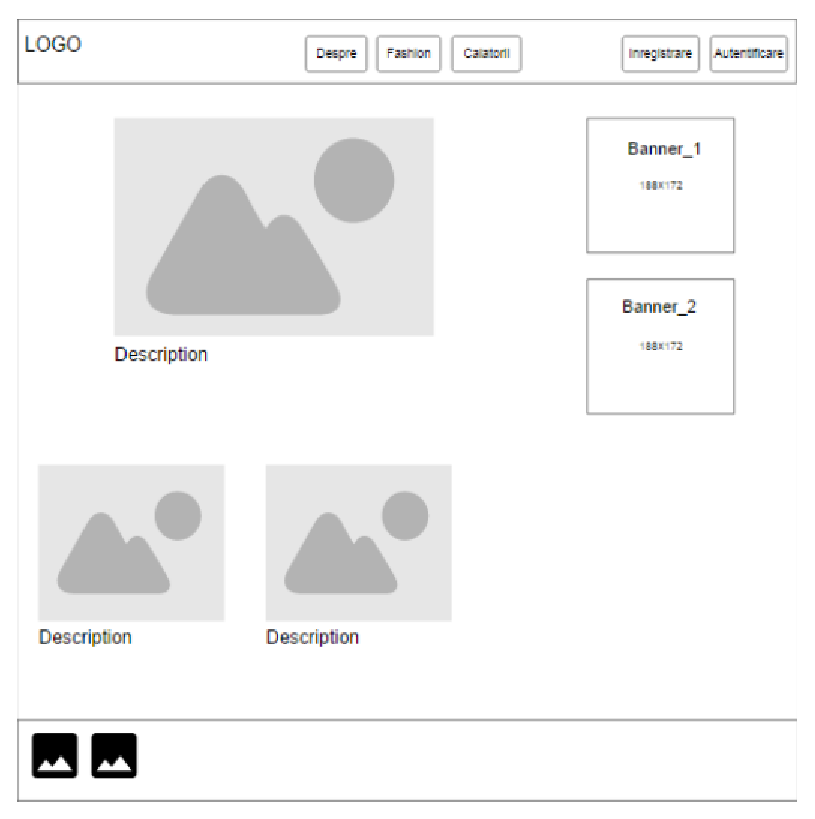
\includegraphics[scale=1]{1}
\end{figure}

\clearpage
\tab Urmatorul pas este de a ne conecta la GitHub folosind o \textbf{cheie SSH}. Initial generam cheia prin introducerea comenzii : \textbf{ssh-keygen -t rsa -b 4096 -C "your-email@example.com" }  , apoi cheia obtinuta o copiem , si in Setarile profilului GitHub cream o cheie in care introducem cheia generata. 
\begin{figure}[h]
\centering
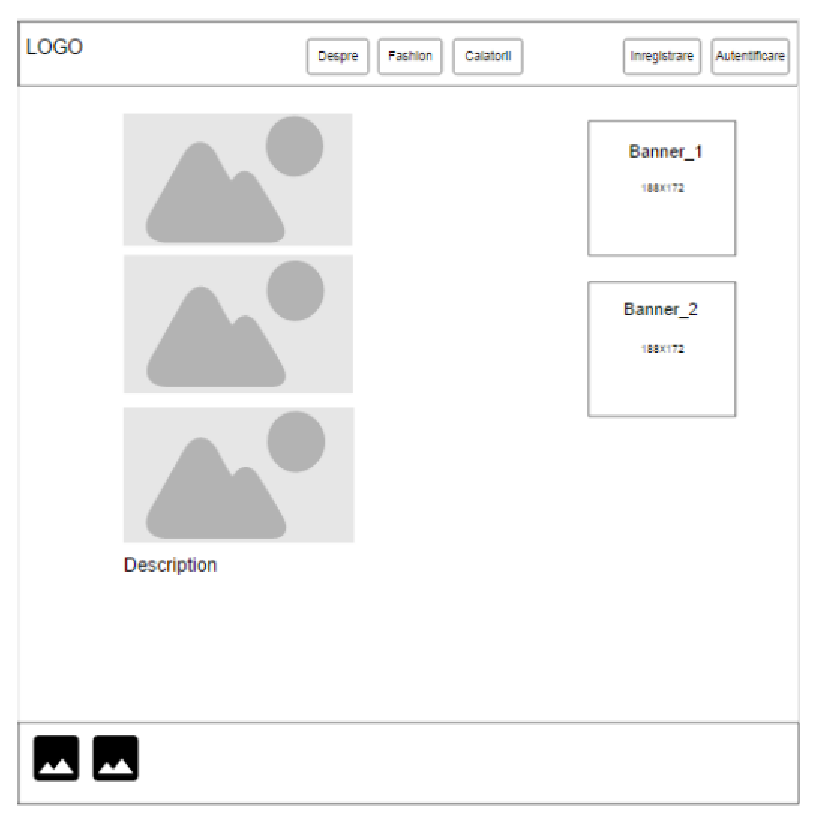
\includegraphics[scale=1]{3}
\end{figure}
\\
\tab Urmatorul pas am clonat repositoriul. Aceasta insemana ca se creaza local pe calculator o copie a repositorului. Pentru aceasta folosim comanda \textbf{git clone SSH URL} (copiat din sectiunea \textbf{Clone or download} de pe GitHub).
\begin{figure}[h]
\centering
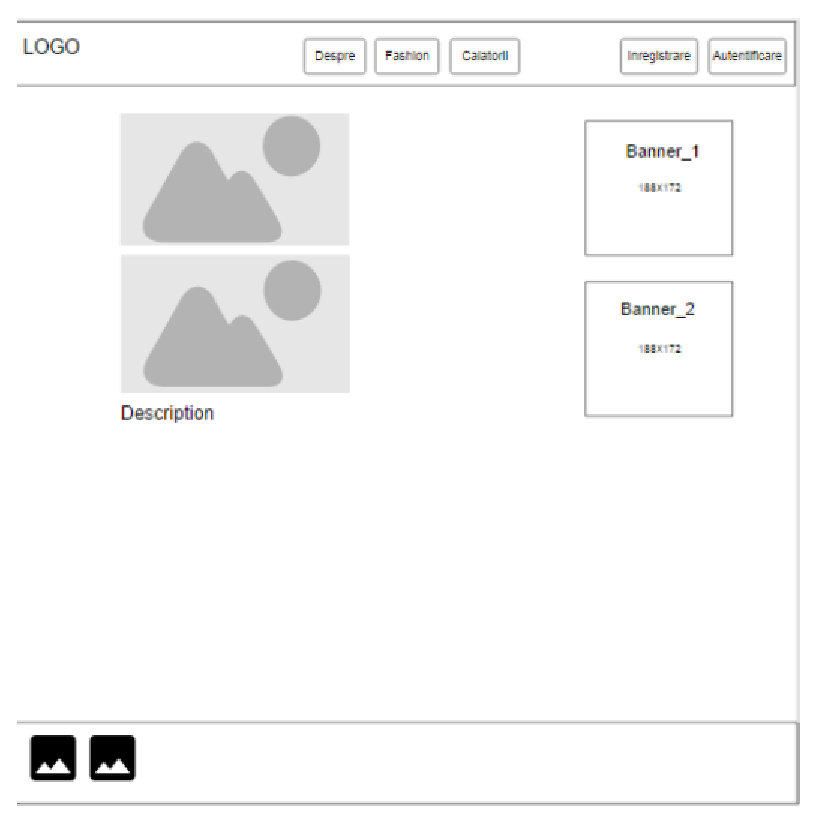
\includegraphics[scale=1]{4}
\end{figure}

\clearpage
\tab Pentru a \textbf{folosi fisierul .gitignore} trebuie sa-l cream in repozitoriu, iar Git il foloseste pentru a determina care fisiere si directorii sa le ignore inainte de a face commit. Am creat si niste fisiere pe care .gitignore le va ignora, pentru a demonstra astfel functionalitatea acestuia. Am creat inca un fisier unde voi duce evidenta commit-urilor , si care il voi modifica cu informatia necesara inaintea fiecarui commit. Comezii folosite: \\
\textbf{touch .gitignore} - pentru fisierului fara denumire ce va avea extensia gitignore iar in acest fisier vom adauga fisierele/directoarele noastre pe care nu le vrem urmarite\\
\textbf{git status} - pentru a verifica daca un fisier urmarit a fost modificat , i s-au adus modificari in continutul acestuia\\
\begin{figure}[h]
\centering
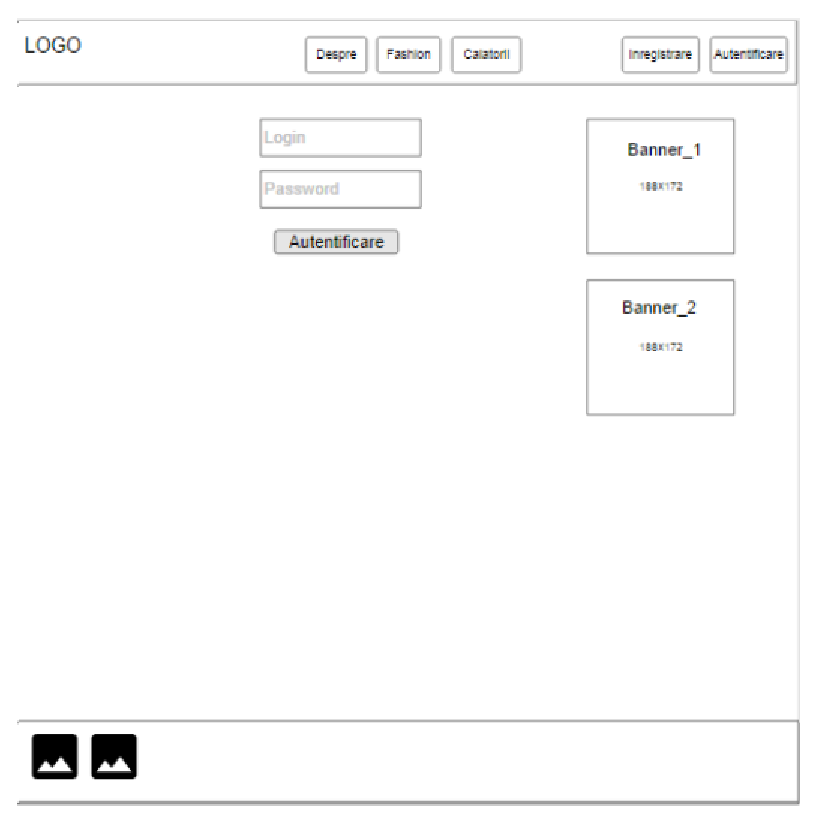
\includegraphics[scale=1]{5}
\end{figure}

\clearpage